\subsection[The Boyer Moore Algorithm]{The Boyer Moore}
    \subsubsection{Introduction \& Application}
        \begin{itemize}
            \item \textbf{Core idea:} The Boyer Moore Algorithm is a practical method to find patterns. This algorithm is the combination of three main ideas comprising scanning the pattern in revserse order, bad character heuristic and good suffix heuristic. This speeds up the searching process
             considerably by skipping a plenty of characters. 
            \item \textbf{Reality applications:}
            \begin{itemize}
                \item Text Editors: Using in "Search" or "Find and Replace" features to locate the destination of the words.
                \item Intrusion Detection Systems (Network Security): use Boyer-Moore to scan network traffic in real-time for "malicious signatures"—specific byte patterns that indicate a cyberattack or virus.
                \item Large-Scale Plagiarism Detection: compare submitted essays against billions of web pages and academic journals to find copied content.
            \end{itemize}
        \end{itemize}

\subsubsection{Pseudocode}
\textbf{Notation:}
\begin{itemize}
    \item \textbf{Text $T$ ($R$ rows, $C$ columns)}: The 2D character matrix.
    \item \textbf{Pattern $P$ ($K$ keywords)}: The list of strings to search.
    \item \textbf{Heuristics}: $BC$ (Bad Character table) and $GS$ (Good Suffix table).
\end{itemize}\textsc{Boyer-Moore Algorithm}($T, P, K, R, C$)
\begin{algorithmic}[1]
    \State $pos = \text{empty array of size } K$
    \For{$idx = 1$ \textbf{to} $K$}
    \State $P_i = P[idx]$, $m = P_i.length$
    \State $BC = \text{PreProcessBadChar}(P_i)$\State $GS = 
    \text{PreProcessGoodSuffix}(P_i)$
    \Statex
    \Comment{Horizontal Search (Rows)}
    \For{$r = 0$ \textbf{to} $R-1$}\State $s = 0$
    \While{$s \le C - m$}\State $j = m - 1$\While{$j \ge 0$ \textbf{and} $P_i[j] == T[r, s+j]$}
    \State $j = j - 1$
    \EndWhile
    \If{$j < 0$}\State add $(r, s)$ to $pos[idx]$
    \State $s = s + GS[0]$
    \Else
    \State $s = s + \max(GS[j], j - BC[T[r, s+j]])$
    \EndIf
    \EndWhile
    \EndFor
    \Statex
    \Comment{Vertical Search (Columns)}
    \For{$c = 0$ \textbf{to} $C-1$}
    \State $s = 0$\While{$s \le R - m$}
    \State $j = m - 1$\While{$j \ge 0$ 
    \textbf{and} $P_i[j] == T[s+j, c]$}
    \State $j = j - 1$
    \EndWhile
    \If{$j < 0$}
    \State add $(s, c)$ to $pos[idx]$
    \State $s = s + GS[0]$
    \Else
    \State $s = s + \max(GS[j], j - BC[T[s+j, c]])$
    \EndIf
    \EndWhile
    \EndFor
    \EndFor
    \State 
    \Return $pos$
\end{algorithmic}
\subsubsection{Step-by-step trace}

    \indent \textbf{Notation:}
        \begin{itemize}
            \item \textbf{Text $T$ (length $n$)}: The main text being searched.
            \item \textbf{Pattern $P$}: The string that we are looking for.
            \item \textbf{Shift ($s$)}: The current offset of the text T.
            \item \textbf{Positions ([(start position, end position), \ldots])}: A list storing the indices where a complete match is found.
        \end{itemize}

    \textbf{Example:} text $T = [G, C, A, T, G, C, C, T, A, G]$ and pattern $P = [T, A, T, G]$
    \begin{itemize}
        
        \item Step 1: Build bad character and good suffix tables base on the pattern we are searching for:
    
         \begin{figure}[H]
            \centering
            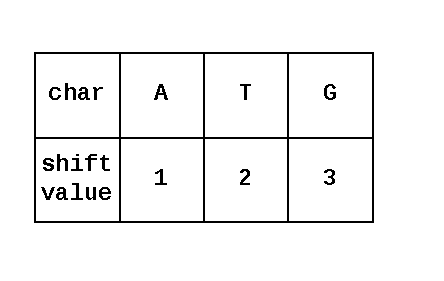
\includegraphics[width=0.4\textwidth, clip]{data/Illustrations/Bad_Char_Table.pdf}
            \caption{Bad character table}
        \end{figure}
        
         \begin{figure}[H]
            \centering
            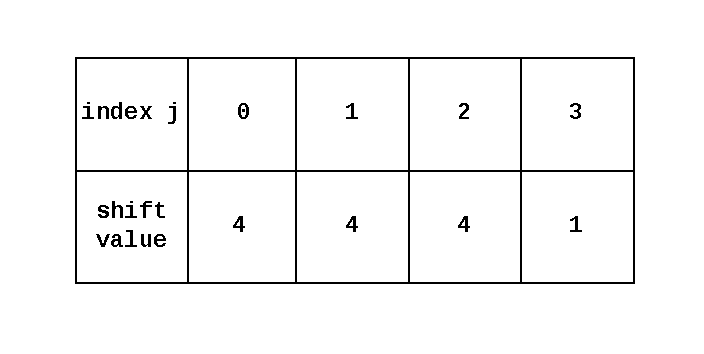
\includegraphics[width=0.5\textwidth, clip]{data/Illustrations/good-suffix-table_cropped.pdf}
            \caption{Good suffix table}
        \end{figure}
        \textbf{Note:}
        \begin{itemize}
            \item \textbf{Bad character table:} Choose the index for characters from 0 to n - 1. In this case, T appears two times, only the last appearance are regconized.
            \item \textbf{Good suffix table:} For index j from 3 to 0, if the suffix of the character at index j is found, the shift value will be decreased. In this example, index 3 is the exception since there is no suffix and the shift value is 1, other suffixes including g, tg, atg are not found in the pattern, then their pattern shifts is the length of the pattern.
        \end{itemize}
        \item Step 2: Compare the patterns and make shifts based on preprocessing values.
         \begin{figure}[H]
            \centering
            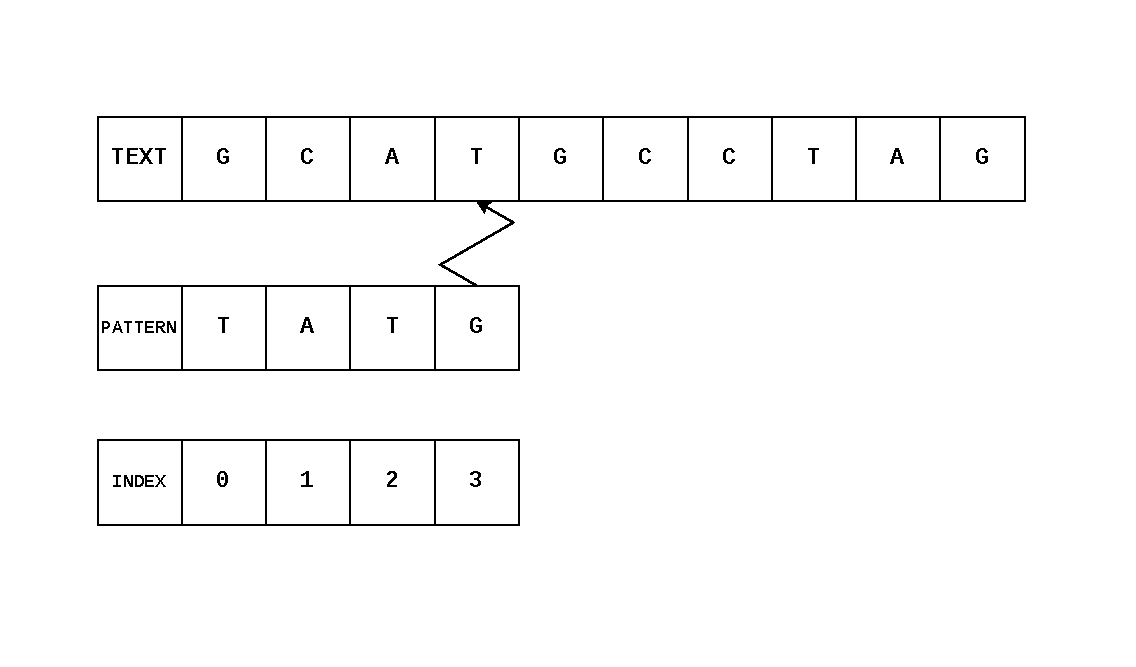
\includegraphics[width=0.75\textwidth, clip]{data/Illustrations/Boyer_moore_step1.pdf}
            \caption{compare pattern from right to left}

        \end{figure}
        Mismatch at index j = 3, then calculate the shift value.

        shift = max(GS, BC)

        GS = 1, BC = max(1, j - lastOccur) = max(1, 3 - 2) = 1 

        $\Rightarrow$ shift value = 1
        
        \item \textbf{Continue searching process}
        \begin{figure}[H]
            \centering
            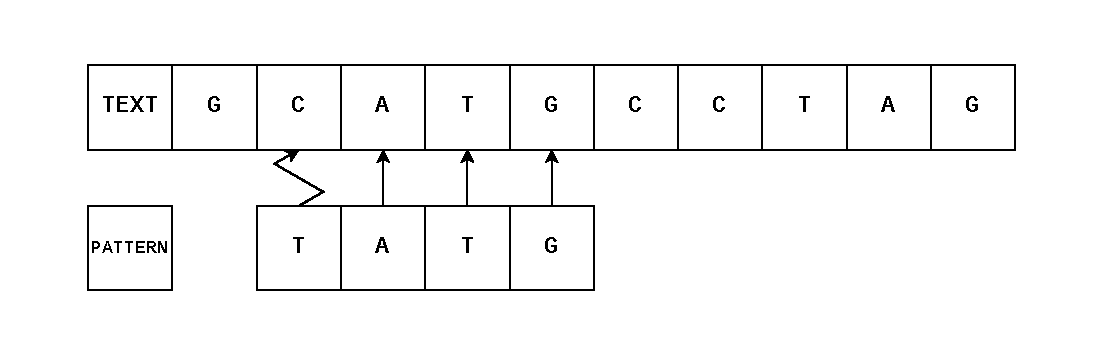
\includegraphics[width=0.75\textwidth, clip]{data/Illustrations/boyer_moore_step2.pdf}
            \caption{compare pattern}

        \end{figure}
        Mismatch at index 0, continue calculate the pattern shift

        Shift value = max(GS, BC) = max(4, 1) = 4

        \item  \textbf{Shift by 4 characters}
        \begin{figure}[H]
            \centering
            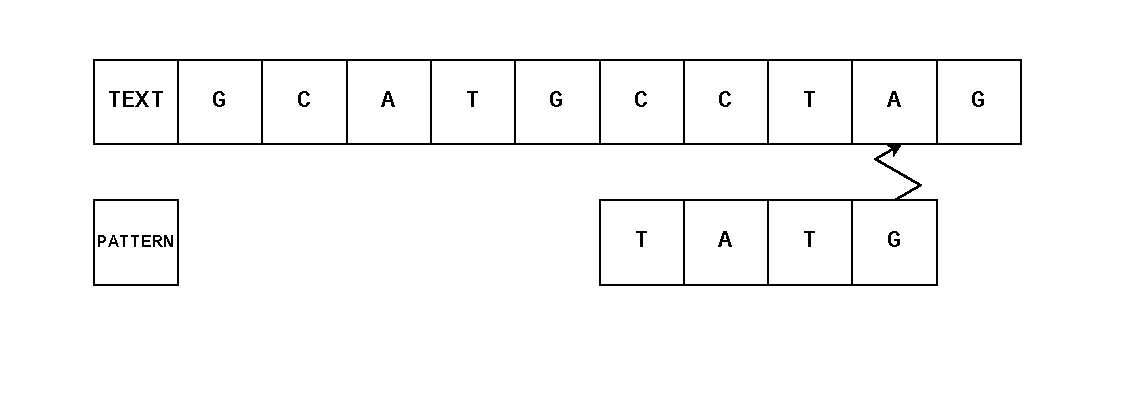
\includegraphics[width=0.75\textwidth, clip]{data/Illustrations/boyer_moore_step3.pdf}
            \caption{Make bigger shift by using good suffix heuristic}

        \end{figure}


       
    \end{itemize}
    

    \subsubsection{Complexity}
        \begin{table}[H]
        \centering
        \renewcommand{\arraystretch}{1.5}
        \begin{tabular}{|l|c|p{8cm}|}
        \hline
        \textbf{Metric} & \textbf{Complexity} & \textbf{Reasoning} \\ \hline
        \textbf{Time (Worst)} & $O(K \cdot m \cdot R \cdot C)$ & Occurs when patterns and text share many prefix characters (e.g., all 'A's). \\ \hline
        \textbf{Time (Average)} & $O(K \cdot R \cdot C)$ & In practice, a mismatch usually occurs after only a few character comparisons. \\ \hline
        \textbf{Time (Best)} & $O(K \cdot R \cdot C)$ & The first character of the pattern always results in a mismatch at every shift. \\ \hline
        \textbf{Auxiliary Space} & $O(1)$ & The algorithm uses only a constant amount of extra memory for loop indices. \\ \hline
        \end{tabular}
        \caption{Complexity Analysis of 2D Brute Force Algorithm}
        \end{table}

    \subsubsection{Discussion}
    \begin{itemize}
        \item In scenarios 1, the number of patterns $K$ is small, and the text is from $10 \times 10$ to $500 \times500$.
        Brute-force approach is efficient and likely linear running time $O(R \cdot C)$.
        \item In scenarios 2, the number of patterns $K$ is large, and the text is fixed at $100 \times 100$.
        This scenario is more challenging for the brute-force approach, as the running time multiplies by $K$ times,
        which is much longer compared to scenario 1.
        \item In conclusion, the brute-force approach is more suitable for scenarios with a small number of patterns.
        It is worse for scenarios with a large number of one.
    \end{itemize}
        